% Created by tikzDevice version 0.12.3 on 2019-09-28 14:19:26
% !TEX encoding = UTF-8 Unicode
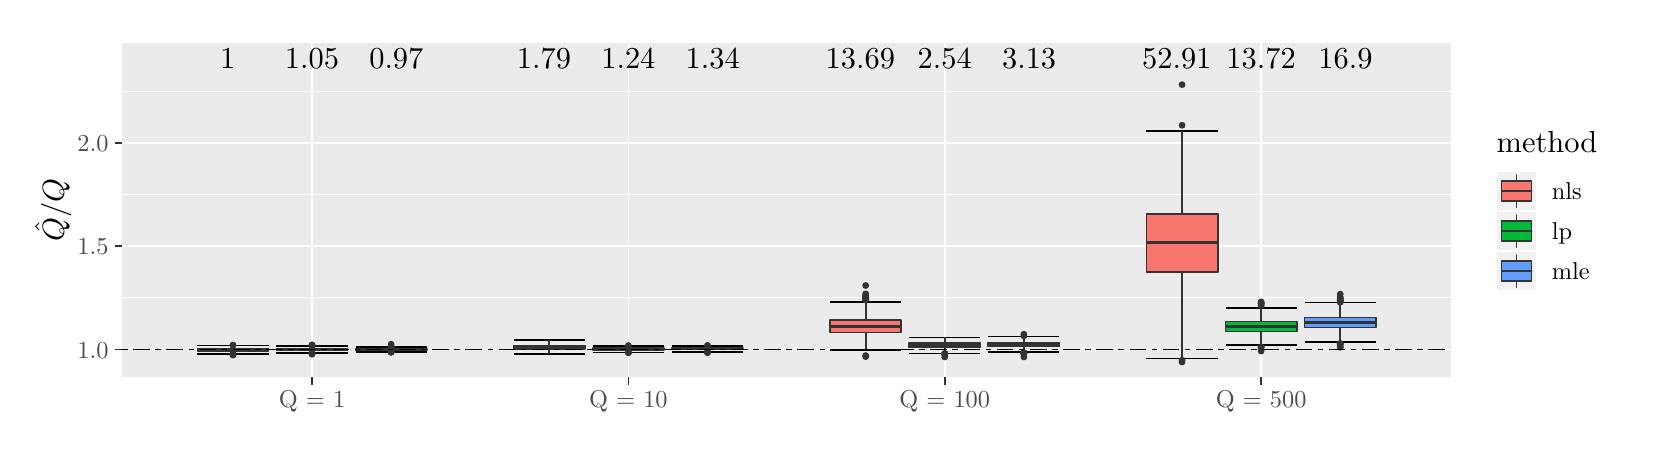
\begin{tikzpicture}[x=1pt,y=1pt]
\definecolor{fillColor}{RGB}{255,255,255}
\path[use as bounding box,fill=fillColor,fill opacity=0.00] (0,0) rectangle (578.16,144.54);
\begin{scope}
\path[clip] (  0.00,  0.00) rectangle (578.16,144.54);
\definecolor{drawColor}{RGB}{255,255,255}
\definecolor{fillColor}{RGB}{255,255,255}

\path[draw=drawColor,line width= 0.6pt,line join=round,line cap=round,fill=fillColor] (  0.00,  0.00) rectangle (578.16,144.54);
\end{scope}
\begin{scope}
\path[clip] ( 34.16, 18.22) rectangle (514.31,139.04);
\definecolor{fillColor}{gray}{0.92}

\path[fill=fillColor] ( 34.16, 18.22) rectangle (514.31,139.04);
\definecolor{drawColor}{RGB}{255,255,255}

\path[draw=drawColor,line width= 0.3pt,line join=round] ( 34.16, 46.89) --
	(514.31, 46.89);

\path[draw=drawColor,line width= 0.3pt,line join=round] ( 34.16, 84.26) --
	(514.31, 84.26);

\path[draw=drawColor,line width= 0.3pt,line join=round] ( 34.16,121.63) --
	(514.31,121.63);

\path[draw=drawColor,line width= 0.6pt,line join=round] ( 34.16, 28.20) --
	(514.31, 28.20);

\path[draw=drawColor,line width= 0.6pt,line join=round] ( 34.16, 65.58) --
	(514.31, 65.58);

\path[draw=drawColor,line width= 0.6pt,line join=round] ( 34.16,102.95) --
	(514.31,102.95);

\path[draw=drawColor,line width= 0.6pt,line join=round] (102.75, 18.22) --
	(102.75,139.04);

\path[draw=drawColor,line width= 0.6pt,line join=round] (217.07, 18.22) --
	(217.07,139.04);

\path[draw=drawColor,line width= 0.6pt,line join=round] (331.39, 18.22) --
	(331.39,139.04);

\path[draw=drawColor,line width= 0.6pt,line join=round] (445.71, 18.22) --
	(445.71,139.04);
\definecolor{drawColor}{RGB}{0,0,0}

\path[draw=drawColor,line width= 0.6pt,line join=round] ( 61.31, 29.72) --
	( 87.03, 29.72);

\path[draw=drawColor,line width= 0.6pt,line join=round] ( 74.17, 29.72) --
	( 74.17, 26.63);

\path[draw=drawColor,line width= 0.6pt,line join=round] ( 61.31, 26.63) --
	( 87.03, 26.63);

\path[draw=drawColor,line width= 0.6pt,line join=round] ( 89.89, 29.45) --
	(115.61, 29.45);

\path[draw=drawColor,line width= 0.6pt,line join=round] (102.75, 29.45) --
	(102.75, 26.99);

\path[draw=drawColor,line width= 0.6pt,line join=round] ( 89.89, 26.99) --
	(115.61, 26.99);

\path[draw=drawColor,line width= 0.6pt,line join=round] (118.47, 29.08) --
	(144.19, 29.08);

\path[draw=drawColor,line width= 0.6pt,line join=round] (131.33, 29.08) --
	(131.33, 27.44);

\path[draw=drawColor,line width= 0.6pt,line join=round] (118.47, 27.44) --
	(144.19, 27.44);

\path[draw=drawColor,line width= 0.6pt,line join=round] (175.63, 31.63) --
	(201.35, 31.63);

\path[draw=drawColor,line width= 0.6pt,line join=round] (188.49, 31.63) --
	(188.49, 26.70);

\path[draw=drawColor,line width= 0.6pt,line join=round] (175.63, 26.70) --
	(201.35, 26.70);

\path[draw=drawColor,line width= 0.6pt,line join=round] (204.21, 29.57) --
	(229.93, 29.57);

\path[draw=drawColor,line width= 0.6pt,line join=round] (217.07, 29.57) --
	(217.07, 27.21);

\path[draw=drawColor,line width= 0.6pt,line join=round] (204.21, 27.21) --
	(229.93, 27.21);

\path[draw=drawColor,line width= 0.6pt,line join=round] (232.79, 29.63) --
	(258.51, 29.63);

\path[draw=drawColor,line width= 0.6pt,line join=round] (245.65, 29.63) --
	(245.65, 27.32);

\path[draw=drawColor,line width= 0.6pt,line join=round] (232.79, 27.32) --
	(258.51, 27.32);

\path[draw=drawColor,line width= 0.6pt,line join=round] (289.95, 45.34) --
	(315.67, 45.34);

\path[draw=drawColor,line width= 0.6pt,line join=round] (302.81, 45.34) --
	(302.81, 28.17);

\path[draw=drawColor,line width= 0.6pt,line join=round] (289.95, 28.17) --
	(315.67, 28.17);

\path[draw=drawColor,line width= 0.6pt,line join=round] (318.53, 32.60) --
	(344.25, 32.60);

\path[draw=drawColor,line width= 0.6pt,line join=round] (331.39, 32.60) --
	(331.39, 26.81);

\path[draw=drawColor,line width= 0.6pt,line join=round] (318.53, 26.81) --
	(344.25, 26.81);

\path[draw=drawColor,line width= 0.6pt,line join=round] (347.11, 32.95) --
	(372.83, 32.95);

\path[draw=drawColor,line width= 0.6pt,line join=round] (359.97, 32.95) --
	(359.97, 27.24);

\path[draw=drawColor,line width= 0.6pt,line join=round] (347.11, 27.24) --
	(372.83, 27.24);

\path[draw=drawColor,line width= 0.6pt,line join=round] (404.27,107.11) --
	(430.00,107.11);

\path[draw=drawColor,line width= 0.6pt,line join=round] (417.13,107.11) --
	(417.13, 24.99);

\path[draw=drawColor,line width= 0.6pt,line join=round] (404.27, 24.99) --
	(430.00, 24.99);

\path[draw=drawColor,line width= 0.6pt,line join=round] (432.85, 43.15) --
	(458.58, 43.15);

\path[draw=drawColor,line width= 0.6pt,line join=round] (445.71, 43.15) --
	(445.71, 29.93);

\path[draw=drawColor,line width= 0.6pt,line join=round] (432.85, 29.93) --
	(458.58, 29.93);

\path[draw=drawColor,line width= 0.6pt,line join=round] (461.43, 45.18) --
	(487.16, 45.18);

\path[draw=drawColor,line width= 0.6pt,line join=round] (474.29, 45.18) --
	(474.29, 30.85);

\path[draw=drawColor,line width= 0.6pt,line join=round] (461.43, 30.85) --
	(487.16, 30.85);
\definecolor{drawColor}{gray}{0.20}
\definecolor{fillColor}{gray}{0.20}

\path[draw=drawColor,line width= 0.4pt,line join=round,line cap=round,fill=fillColor] ( 74.17, 26.40) circle (  1.02);

\path[draw=drawColor,line width= 0.4pt,line join=round,line cap=round,fill=fillColor] ( 74.17, 29.83) circle (  1.02);

\path[draw=drawColor,line width= 0.4pt,line join=round,line cap=round,fill=fillColor] ( 74.17, 29.77) circle (  1.02);

\path[draw=drawColor,line width= 0.4pt,line join=round,line cap=round,fill=fillColor] ( 74.17, 26.55) circle (  1.02);

\path[draw=drawColor,line width= 0.4pt,line join=round,line cap=round,fill=fillColor] ( 74.17, 26.41) circle (  1.02);

\path[draw=drawColor,line width= 0.4pt,line join=round,line cap=round,fill=fillColor] ( 74.17, 26.21) circle (  1.02);

\path[draw=drawColor,line width= 0.4pt,line join=round,line cap=round,fill=fillColor] ( 74.17, 26.46) circle (  1.02);

\path[draw=drawColor,line width= 0.6pt,line join=round] ( 74.17, 28.57) -- ( 74.17, 29.72);

\path[draw=drawColor,line width= 0.6pt,line join=round] ( 74.17, 27.79) -- ( 74.17, 26.63);
\definecolor{fillColor}{RGB}{248,118,109}

\path[draw=drawColor,line width= 0.6pt,line join=round,line cap=round,fill=fillColor] ( 61.31, 28.57) --
	( 61.31, 27.79) --
	( 87.03, 27.79) --
	( 87.03, 28.57) --
	( 61.31, 28.57) --
	cycle;

\path[draw=drawColor,line width= 1.1pt,line join=round] ( 61.31, 28.22) -- ( 87.03, 28.22);
\definecolor{fillColor}{gray}{0.20}

\path[draw=drawColor,line width= 0.4pt,line join=round,line cap=round,fill=fillColor] (102.75, 26.76) circle (  1.02);

\path[draw=drawColor,line width= 0.4pt,line join=round,line cap=round,fill=fillColor] (102.75, 26.53) circle (  1.02);

\path[draw=drawColor,line width= 0.4pt,line join=round,line cap=round,fill=fillColor] (102.75, 29.57) circle (  1.02);

\path[draw=drawColor,line width= 0.4pt,line join=round,line cap=round,fill=fillColor] (102.75, 29.58) circle (  1.02);

\path[draw=drawColor,line width= 0.4pt,line join=round,line cap=round,fill=fillColor] (102.75, 26.88) circle (  1.02);

\path[draw=drawColor,line width= 0.4pt,line join=round,line cap=round,fill=fillColor] (102.75, 29.74) circle (  1.02);

\path[draw=drawColor,line width= 0.4pt,line join=round,line cap=round,fill=fillColor] (102.75, 26.84) circle (  1.02);

\path[draw=drawColor,line width= 0.4pt,line join=round,line cap=round,fill=fillColor] (102.75, 26.92) circle (  1.02);

\path[draw=drawColor,line width= 0.4pt,line join=round,line cap=round,fill=fillColor] (102.75, 26.79) circle (  1.02);

\path[draw=drawColor,line width= 0.4pt,line join=round,line cap=round,fill=fillColor] (102.75, 29.94) circle (  1.02);

\path[draw=drawColor,line width= 0.6pt,line join=round] (102.75, 28.56) -- (102.75, 29.45);

\path[draw=drawColor,line width= 0.6pt,line join=round] (102.75, 27.92) -- (102.75, 26.99);
\definecolor{fillColor}{RGB}{0,186,56}

\path[draw=drawColor,line width= 0.6pt,line join=round,line cap=round,fill=fillColor] ( 89.89, 28.56) --
	( 89.89, 27.92) --
	(115.61, 27.92) --
	(115.61, 28.56) --
	( 89.89, 28.56) --
	cycle;

\path[draw=drawColor,line width= 1.1pt,line join=round] ( 89.89, 28.26) -- (115.61, 28.26);
\definecolor{fillColor}{gray}{0.20}

\path[draw=drawColor,line width= 0.4pt,line join=round,line cap=round,fill=fillColor] (131.33, 27.38) circle (  1.02);

\path[draw=drawColor,line width= 0.4pt,line join=round,line cap=round,fill=fillColor] (131.33, 27.34) circle (  1.02);

\path[draw=drawColor,line width= 0.4pt,line join=round,line cap=round,fill=fillColor] (131.33, 29.26) circle (  1.02);

\path[draw=drawColor,line width= 0.4pt,line join=round,line cap=round,fill=fillColor] (131.33, 27.28) circle (  1.02);

\path[draw=drawColor,line width= 0.4pt,line join=round,line cap=round,fill=fillColor] (131.33, 29.13) circle (  1.02);

\path[draw=drawColor,line width= 0.4pt,line join=round,line cap=round,fill=fillColor] (131.33, 30.15) circle (  1.02);

\path[draw=drawColor,line width= 0.4pt,line join=round,line cap=round,fill=fillColor] (131.33, 27.36) circle (  1.02);

\path[draw=drawColor,line width= 0.4pt,line join=round,line cap=round,fill=fillColor] (131.33, 27.35) circle (  1.02);

\path[draw=drawColor,line width= 0.4pt,line join=round,line cap=round,fill=fillColor] (131.33, 29.32) circle (  1.02);

\path[draw=drawColor,line width= 0.4pt,line join=round,line cap=round,fill=fillColor] (131.33, 27.36) circle (  1.02);

\path[draw=drawColor,line width= 0.6pt,line join=round] (131.33, 28.47) -- (131.33, 29.08);

\path[draw=drawColor,line width= 0.6pt,line join=round] (131.33, 28.05) -- (131.33, 27.44);
\definecolor{fillColor}{RGB}{97,156,255}

\path[draw=drawColor,line width= 0.6pt,line join=round,line cap=round,fill=fillColor] (118.47, 28.47) --
	(118.47, 28.05) --
	(144.19, 28.05) --
	(144.19, 28.47) --
	(118.47, 28.47) --
	cycle;

\path[draw=drawColor,line width= 1.1pt,line join=round] (118.47, 28.23) -- (144.19, 28.23);

\path[draw=drawColor,line width= 0.6pt,line join=round] (188.49, 29.75) -- (188.49, 31.63);

\path[draw=drawColor,line width= 0.6pt,line join=round] (188.49, 28.48) -- (188.49, 26.70);
\definecolor{fillColor}{RGB}{248,118,109}

\path[draw=drawColor,line width= 0.6pt,line join=round,line cap=round,fill=fillColor] (175.63, 29.75) --
	(175.63, 28.48) --
	(201.35, 28.48) --
	(201.35, 29.75) --
	(175.63, 29.75) --
	cycle;

\path[draw=drawColor,line width= 1.1pt,line join=round] (175.63, 29.07) -- (201.35, 29.07);
\definecolor{fillColor}{gray}{0.20}

\path[draw=drawColor,line width= 0.4pt,line join=round,line cap=round,fill=fillColor] (217.07, 27.18) circle (  1.02);

\path[draw=drawColor,line width= 0.4pt,line join=round,line cap=round,fill=fillColor] (217.07, 29.67) circle (  1.02);

\path[draw=drawColor,line width= 0.4pt,line join=round,line cap=round,fill=fillColor] (217.07, 27.15) circle (  1.02);

\path[draw=drawColor,line width= 0.4pt,line join=round,line cap=round,fill=fillColor] (217.07, 27.15) circle (  1.02);

\path[draw=drawColor,line width= 0.6pt,line join=round] (217.07, 28.71) -- (217.07, 29.57);

\path[draw=drawColor,line width= 0.6pt,line join=round] (217.07, 28.10) -- (217.07, 27.21);
\definecolor{fillColor}{RGB}{0,186,56}

\path[draw=drawColor,line width= 0.6pt,line join=round,line cap=round,fill=fillColor] (204.21, 28.71) --
	(204.21, 28.10) --
	(229.93, 28.10) --
	(229.93, 28.71) --
	(204.21, 28.71) --
	cycle;

\path[draw=drawColor,line width= 1.1pt,line join=round] (204.21, 28.40) -- (229.93, 28.40);
\definecolor{fillColor}{gray}{0.20}

\path[draw=drawColor,line width= 0.4pt,line join=round,line cap=round,fill=fillColor] (245.65, 27.27) circle (  1.02);

\path[draw=drawColor,line width= 0.4pt,line join=round,line cap=round,fill=fillColor] (245.65, 29.67) circle (  1.02);

\path[draw=drawColor,line width= 0.4pt,line join=round,line cap=round,fill=fillColor] (245.65, 27.27) circle (  1.02);

\path[draw=drawColor,line width= 0.4pt,line join=round,line cap=round,fill=fillColor] (245.65, 27.13) circle (  1.02);

\path[draw=drawColor,line width= 0.4pt,line join=round,line cap=round,fill=fillColor] (245.65, 27.25) circle (  1.02);

\path[draw=drawColor,line width= 0.4pt,line join=round,line cap=round,fill=fillColor] (245.65, 27.30) circle (  1.02);

\path[draw=drawColor,line width= 0.4pt,line join=round,line cap=round,fill=fillColor] (245.65, 27.30) circle (  1.02);

\path[draw=drawColor,line width= 0.4pt,line join=round,line cap=round,fill=fillColor] (245.65, 29.70) circle (  1.02);

\path[draw=drawColor,line width= 0.4pt,line join=round,line cap=round,fill=fillColor] (245.65, 27.27) circle (  1.02);

\path[draw=drawColor,line width= 0.6pt,line join=round] (245.65, 28.77) -- (245.65, 29.63);

\path[draw=drawColor,line width= 0.6pt,line join=round] (245.65, 28.19) -- (245.65, 27.32);
\definecolor{fillColor}{RGB}{97,156,255}

\path[draw=drawColor,line width= 0.6pt,line join=round,line cap=round,fill=fillColor] (232.79, 28.77) --
	(232.79, 28.19) --
	(258.51, 28.19) --
	(258.51, 28.77) --
	(232.79, 28.77) --
	cycle;

\path[draw=drawColor,line width= 1.1pt,line join=round] (232.79, 28.45) -- (258.51, 28.45);
\definecolor{fillColor}{gray}{0.20}

\path[draw=drawColor,line width= 0.4pt,line join=round,line cap=round,fill=fillColor] (302.81, 48.36) circle (  1.02);

\path[draw=drawColor,line width= 0.4pt,line join=round,line cap=round,fill=fillColor] (302.81, 46.16) circle (  1.02);

\path[draw=drawColor,line width= 0.4pt,line join=round,line cap=round,fill=fillColor] (302.81, 46.82) circle (  1.02);

\path[draw=drawColor,line width= 0.4pt,line join=round,line cap=round,fill=fillColor] (302.81, 25.68) circle (  1.02);

\path[draw=drawColor,line width= 0.4pt,line join=round,line cap=round,fill=fillColor] (302.81, 46.18) circle (  1.02);

\path[draw=drawColor,line width= 0.4pt,line join=round,line cap=round,fill=fillColor] (302.81, 26.05) circle (  1.02);

\path[draw=drawColor,line width= 0.4pt,line join=round,line cap=round,fill=fillColor] (302.81, 47.62) circle (  1.02);

\path[draw=drawColor,line width= 0.4pt,line join=round,line cap=round,fill=fillColor] (302.81, 46.77) circle (  1.02);

\path[draw=drawColor,line width= 0.4pt,line join=round,line cap=round,fill=fillColor] (302.81, 51.37) circle (  1.02);

\path[draw=drawColor,line width= 0.4pt,line join=round,line cap=round,fill=fillColor] (302.81, 46.72) circle (  1.02);

\path[draw=drawColor,line width= 0.4pt,line join=round,line cap=round,fill=fillColor] (302.81, 47.23) circle (  1.02);

\path[draw=drawColor,line width= 0.4pt,line join=round,line cap=round,fill=fillColor] (302.81, 47.65) circle (  1.02);

\path[draw=drawColor,line width= 0.6pt,line join=round] (302.81, 38.97) -- (302.81, 45.34);

\path[draw=drawColor,line width= 0.6pt,line join=round] (302.81, 34.33) -- (302.81, 28.17);
\definecolor{fillColor}{RGB}{248,118,109}

\path[draw=drawColor,line width= 0.6pt,line join=round,line cap=round,fill=fillColor] (289.95, 38.97) --
	(289.95, 34.33) --
	(315.67, 34.33) --
	(315.67, 38.97) --
	(289.95, 38.97) --
	cycle;

\path[draw=drawColor,line width= 1.1pt,line join=round] (289.95, 36.72) -- (315.67, 36.72);
\definecolor{fillColor}{gray}{0.20}

\path[draw=drawColor,line width= 0.4pt,line join=round,line cap=round,fill=fillColor] (331.39, 26.58) circle (  1.02);

\path[draw=drawColor,line width= 0.4pt,line join=round,line cap=round,fill=fillColor] (331.39, 25.56) circle (  1.02);

\path[draw=drawColor,line width= 0.4pt,line join=round,line cap=round,fill=fillColor] (331.39, 26.65) circle (  1.02);

\path[draw=drawColor,line width= 0.4pt,line join=round,line cap=round,fill=fillColor] (331.39, 26.77) circle (  1.02);

\path[draw=drawColor,line width= 0.4pt,line join=round,line cap=round,fill=fillColor] (331.39, 26.73) circle (  1.02);

\path[draw=drawColor,line width= 0.4pt,line join=round,line cap=round,fill=fillColor] (331.39, 26.78) circle (  1.02);

\path[draw=drawColor,line width= 0.4pt,line join=round,line cap=round,fill=fillColor] (331.39, 26.50) circle (  1.02);

\path[draw=drawColor,line width= 0.6pt,line join=round] (331.39, 30.48) -- (331.39, 32.60);

\path[draw=drawColor,line width= 0.6pt,line join=round] (331.39, 29.00) -- (331.39, 26.81);
\definecolor{fillColor}{RGB}{0,186,56}

\path[draw=drawColor,line width= 0.6pt,line join=round,line cap=round,fill=fillColor] (318.53, 30.48) --
	(318.53, 29.00) --
	(344.25, 29.00) --
	(344.25, 30.48) --
	(318.53, 30.48) --
	cycle;

\path[draw=drawColor,line width= 1.1pt,line join=round] (318.53, 29.83) -- (344.25, 29.83);
\definecolor{fillColor}{gray}{0.20}

\path[draw=drawColor,line width= 0.4pt,line join=round,line cap=round,fill=fillColor] (359.97, 33.77) circle (  1.02);

\path[draw=drawColor,line width= 0.4pt,line join=round,line cap=round,fill=fillColor] (359.97, 26.95) circle (  1.02);

\path[draw=drawColor,line width= 0.4pt,line join=round,line cap=round,fill=fillColor] (359.97, 25.55) circle (  1.02);

\path[draw=drawColor,line width= 0.4pt,line join=round,line cap=round,fill=fillColor] (359.97, 27.02) circle (  1.02);

\path[draw=drawColor,line width= 0.4pt,line join=round,line cap=round,fill=fillColor] (359.97, 27.08) circle (  1.02);

\path[draw=drawColor,line width= 0.4pt,line join=round,line cap=round,fill=fillColor] (359.97, 26.87) circle (  1.02);

\path[draw=drawColor,line width= 0.4pt,line join=round,line cap=round,fill=fillColor] (359.97, 27.03) circle (  1.02);

\path[draw=drawColor,line width= 0.4pt,line join=round,line cap=round,fill=fillColor] (359.97, 33.13) circle (  1.02);

\path[draw=drawColor,line width= 0.4pt,line join=round,line cap=round,fill=fillColor] (359.97, 26.58) circle (  1.02);

\path[draw=drawColor,line width= 0.6pt,line join=round] (359.97, 30.80) -- (359.97, 32.95);

\path[draw=drawColor,line width= 0.6pt,line join=round] (359.97, 29.36) -- (359.97, 27.24);
\definecolor{fillColor}{RGB}{97,156,255}

\path[draw=drawColor,line width= 0.6pt,line join=round,line cap=round,fill=fillColor] (347.11, 30.80) --
	(347.11, 29.36) --
	(372.83, 29.36) --
	(372.83, 30.80) --
	(347.11, 30.80) --
	cycle;

\path[draw=drawColor,line width= 1.1pt,line join=round] (347.11, 30.15) -- (372.83, 30.15);
\definecolor{fillColor}{gray}{0.20}

\path[draw=drawColor,line width= 0.4pt,line join=round,line cap=round,fill=fillColor] (417.13, 24.38) circle (  1.02);

\path[draw=drawColor,line width= 0.4pt,line join=round,line cap=round,fill=fillColor] (417.13,109.28) circle (  1.02);

\path[draw=drawColor,line width= 0.4pt,line join=round,line cap=round,fill=fillColor] (417.13, 23.71) circle (  1.02);

\path[draw=drawColor,line width= 0.4pt,line join=round,line cap=round,fill=fillColor] (417.13,123.97) circle (  1.02);

\path[draw=drawColor,line width= 0.6pt,line join=round] (417.13, 77.16) -- (417.13,107.11);

\path[draw=drawColor,line width= 0.6pt,line join=round] (417.13, 56.27) -- (417.13, 24.99);
\definecolor{fillColor}{RGB}{248,118,109}

\path[draw=drawColor,line width= 0.6pt,line join=round,line cap=round,fill=fillColor] (404.27, 77.16) --
	(404.27, 56.27) --
	(430.00, 56.27) --
	(430.00, 77.16) --
	(404.27, 77.16) --
	cycle;

\path[draw=drawColor,line width= 1.1pt,line join=round] (404.27, 67.06) -- (430.00, 67.06);
\definecolor{fillColor}{gray}{0.20}

\path[draw=drawColor,line width= 0.4pt,line join=round,line cap=round,fill=fillColor] (445.71, 45.13) circle (  1.02);

\path[draw=drawColor,line width= 0.4pt,line join=round,line cap=round,fill=fillColor] (445.71, 45.46) circle (  1.02);

\path[draw=drawColor,line width= 0.4pt,line join=round,line cap=round,fill=fillColor] (445.71, 29.10) circle (  1.02);

\path[draw=drawColor,line width= 0.4pt,line join=round,line cap=round,fill=fillColor] (445.71, 44.91) circle (  1.02);

\path[draw=drawColor,line width= 0.4pt,line join=round,line cap=round,fill=fillColor] (445.71, 29.11) circle (  1.02);

\path[draw=drawColor,line width= 0.4pt,line join=round,line cap=round,fill=fillColor] (445.71, 27.68) circle (  1.02);

\path[draw=drawColor,line width= 0.4pt,line join=round,line cap=round,fill=fillColor] (445.71, 45.00) circle (  1.02);

\path[draw=drawColor,line width= 0.4pt,line join=round,line cap=round,fill=fillColor] (445.71, 29.03) circle (  1.02);

\path[draw=drawColor,line width= 0.4pt,line join=round,line cap=round,fill=fillColor] (445.71, 44.09) circle (  1.02);

\path[draw=drawColor,line width= 0.4pt,line join=round,line cap=round,fill=fillColor] (445.71, 44.23) circle (  1.02);

\path[draw=drawColor,line width= 0.4pt,line join=round,line cap=round,fill=fillColor] (445.71, 44.96) circle (  1.02);

\path[draw=drawColor,line width= 0.6pt,line join=round] (445.71, 38.42) -- (445.71, 43.15);

\path[draw=drawColor,line width= 0.6pt,line join=round] (445.71, 34.79) -- (445.71, 29.93);
\definecolor{fillColor}{RGB}{0,186,56}

\path[draw=drawColor,line width= 0.6pt,line join=round,line cap=round,fill=fillColor] (432.85, 38.42) --
	(432.85, 34.79) --
	(458.58, 34.79) --
	(458.58, 38.42) --
	(432.85, 38.42) --
	cycle;

\path[draw=drawColor,line width= 1.1pt,line join=round] (432.85, 36.54) -- (458.58, 36.54);
\definecolor{fillColor}{gray}{0.20}

\path[draw=drawColor,line width= 0.4pt,line join=round,line cap=round,fill=fillColor] (474.29, 29.91) circle (  1.02);

\path[draw=drawColor,line width= 0.4pt,line join=round,line cap=round,fill=fillColor] (474.29, 30.25) circle (  1.02);

\path[draw=drawColor,line width= 0.4pt,line join=round,line cap=round,fill=fillColor] (474.29, 29.12) circle (  1.02);

\path[draw=drawColor,line width= 0.4pt,line join=round,line cap=round,fill=fillColor] (474.29, 29.13) circle (  1.02);

\path[draw=drawColor,line width= 0.4pt,line join=round,line cap=round,fill=fillColor] (474.29, 47.08) circle (  1.02);

\path[draw=drawColor,line width= 0.4pt,line join=round,line cap=round,fill=fillColor] (474.29, 46.92) circle (  1.02);

\path[draw=drawColor,line width= 0.4pt,line join=round,line cap=round,fill=fillColor] (474.29, 30.41) circle (  1.02);

\path[draw=drawColor,line width= 0.4pt,line join=round,line cap=round,fill=fillColor] (474.29, 45.36) circle (  1.02);

\path[draw=drawColor,line width= 0.4pt,line join=round,line cap=round,fill=fillColor] (474.29, 48.26) circle (  1.02);

\path[draw=drawColor,line width= 0.4pt,line join=round,line cap=round,fill=fillColor] (474.29, 46.02) circle (  1.02);

\path[draw=drawColor,line width= 0.4pt,line join=round,line cap=round,fill=fillColor] (474.29, 45.38) circle (  1.02);

\path[draw=drawColor,line width= 0.4pt,line join=round,line cap=round,fill=fillColor] (474.29, 46.32) circle (  1.02);

\path[draw=drawColor,line width= 0.4pt,line join=round,line cap=round,fill=fillColor] (474.29, 30.38) circle (  1.02);

\path[draw=drawColor,line width= 0.4pt,line join=round,line cap=round,fill=fillColor] (474.29, 46.02) circle (  1.02);

\path[draw=drawColor,line width= 0.6pt,line join=round] (474.29, 39.78) -- (474.29, 45.18);

\path[draw=drawColor,line width= 0.6pt,line join=round] (474.29, 36.16) -- (474.29, 30.85);
\definecolor{fillColor}{RGB}{97,156,255}

\path[draw=drawColor,line width= 0.6pt,line join=round,line cap=round,fill=fillColor] (461.43, 39.78) --
	(461.43, 36.16) --
	(487.16, 36.16) --
	(487.16, 39.78) --
	(461.43, 39.78) --
	cycle;

\path[draw=drawColor,line width= 1.1pt,line join=round] (461.43, 37.94) -- (487.16, 37.94);
\definecolor{drawColor}{RGB}{0,0,0}

\path[draw=drawColor,line width= 0.6pt,dash pattern=on 2pt off 2pt on 6pt off 2pt ,line join=round] ( 34.16, 28.20) -- (514.31, 28.20);

\node[text=drawColor,anchor=base,inner sep=0pt, outer sep=0pt, scale=  1.10] at (133.23,129.75) {0.97};

\node[text=drawColor,anchor=base,inner sep=0pt, outer sep=0pt, scale=  1.10] at (102.75,129.75) {1.05};

\node[text=drawColor,anchor=base,inner sep=0pt, outer sep=0pt, scale=  1.10] at ( 72.26,129.75) {1};

\node[text=drawColor,anchor=base,inner sep=0pt, outer sep=0pt, scale=  1.10] at (247.56,129.75) {1.34};

\node[text=drawColor,anchor=base,inner sep=0pt, outer sep=0pt, scale=  1.10] at (217.07,129.75) {1.24};

\node[text=drawColor,anchor=base,inner sep=0pt, outer sep=0pt, scale=  1.10] at (186.59,129.75) {1.79};

\node[text=drawColor,anchor=base,inner sep=0pt, outer sep=0pt, scale=  1.10] at (361.88,129.75) {3.13};

\node[text=drawColor,anchor=base,inner sep=0pt, outer sep=0pt, scale=  1.10] at (331.39,129.75) {2.54};

\node[text=drawColor,anchor=base,inner sep=0pt, outer sep=0pt, scale=  1.10] at (300.91,129.75) {13.69};

\node[text=drawColor,anchor=base,inner sep=0pt, outer sep=0pt, scale=  1.10] at (476.20,129.75) {16.9};

\node[text=drawColor,anchor=base,inner sep=0pt, outer sep=0pt, scale=  1.10] at (445.71,129.75) {13.72};

\node[text=drawColor,anchor=base,inner sep=0pt, outer sep=0pt, scale=  1.10] at (415.23,129.75) {52.91};
\end{scope}
\begin{scope}
\path[clip] (  0.00,  0.00) rectangle (578.16,144.54);
\definecolor{drawColor}{gray}{0.30}

\node[text=drawColor,anchor=base east,inner sep=0pt, outer sep=0pt, scale=  0.88] at ( 29.21, 25.17) {1.0};

\node[text=drawColor,anchor=base east,inner sep=0pt, outer sep=0pt, scale=  0.88] at ( 29.21, 62.54) {1.5};

\node[text=drawColor,anchor=base east,inner sep=0pt, outer sep=0pt, scale=  0.88] at ( 29.21, 99.92) {2.0};
\end{scope}
\begin{scope}
\path[clip] (  0.00,  0.00) rectangle (578.16,144.54);
\definecolor{drawColor}{gray}{0.20}

\path[draw=drawColor,line width= 0.6pt,line join=round] ( 31.41, 28.20) --
	( 34.16, 28.20);

\path[draw=drawColor,line width= 0.6pt,line join=round] ( 31.41, 65.58) --
	( 34.16, 65.58);

\path[draw=drawColor,line width= 0.6pt,line join=round] ( 31.41,102.95) --
	( 34.16,102.95);
\end{scope}
\begin{scope}
\path[clip] (  0.00,  0.00) rectangle (578.16,144.54);
\definecolor{drawColor}{gray}{0.20}

\path[draw=drawColor,line width= 0.6pt,line join=round] (102.75, 15.47) --
	(102.75, 18.22);

\path[draw=drawColor,line width= 0.6pt,line join=round] (217.07, 15.47) --
	(217.07, 18.22);

\path[draw=drawColor,line width= 0.6pt,line join=round] (331.39, 15.47) --
	(331.39, 18.22);

\path[draw=drawColor,line width= 0.6pt,line join=round] (445.71, 15.47) --
	(445.71, 18.22);
\end{scope}
\begin{scope}
\path[clip] (  0.00,  0.00) rectangle (578.16,144.54);
\definecolor{drawColor}{gray}{0.30}

\node[text=drawColor,anchor=base,inner sep=0pt, outer sep=0pt, scale=  0.88] at (102.75,  7.21) {Q = 1};

\node[text=drawColor,anchor=base,inner sep=0pt, outer sep=0pt, scale=  0.88] at (217.07,  7.21) {Q = 10};

\node[text=drawColor,anchor=base,inner sep=0pt, outer sep=0pt, scale=  0.88] at (331.39,  7.21) {Q = 100};

\node[text=drawColor,anchor=base,inner sep=0pt, outer sep=0pt, scale=  0.88] at (445.71,  7.21) {Q = 500};
\end{scope}
\begin{scope}
\path[clip] (  0.00,  0.00) rectangle (578.16,144.54);
\definecolor{drawColor}{RGB}{0,0,0}

\node[text=drawColor,rotate= 90.00,anchor=base,inner sep=0pt, outer sep=0pt, scale=  1.10] at ( 13.08, 78.63) {$\hat{Q}/Q$};
\end{scope}
\begin{scope}
\path[clip] (  0.00,  0.00) rectangle (578.16,144.54);
\definecolor{fillColor}{RGB}{255,255,255}

\path[fill=fillColor] (525.31, 43.84) rectangle (572.66,113.42);
\end{scope}
\begin{scope}
\path[clip] (  0.00,  0.00) rectangle (578.16,144.54);
\definecolor{drawColor}{RGB}{0,0,0}

\node[text=drawColor,anchor=base west,inner sep=0pt, outer sep=0pt, scale=  1.10] at (530.81, 99.27) {method};
\end{scope}
\begin{scope}
\path[clip] (  0.00,  0.00) rectangle (578.16,144.54);
\definecolor{drawColor}{RGB}{255,255,255}
\definecolor{fillColor}{gray}{0.95}

\path[draw=drawColor,line width= 0.6pt,line join=round,line cap=round,fill=fillColor] (530.81, 78.25) rectangle (545.26, 92.70);
\end{scope}
\begin{scope}
\path[clip] (  0.00,  0.00) rectangle (578.16,144.54);
\definecolor{drawColor}{gray}{0.20}

\path[draw=drawColor,line width= 0.6pt,line join=round,line cap=round] (538.03, 79.70) --
	(538.03, 81.86);

\path[draw=drawColor,line width= 0.6pt,line join=round,line cap=round] (538.03, 89.09) --
	(538.03, 91.26);
\definecolor{fillColor}{RGB}{248,118,109}

\path[draw=drawColor,line width= 0.6pt,line join=round,line cap=round,fill=fillColor] (532.61, 81.86) rectangle (543.45, 89.09);

\path[draw=drawColor,line width= 0.6pt,line join=round,line cap=round] (532.61, 85.48) --
	(543.45, 85.48);
\end{scope}
\begin{scope}
\path[clip] (  0.00,  0.00) rectangle (578.16,144.54);
\definecolor{drawColor}{RGB}{255,255,255}
\definecolor{fillColor}{gray}{0.95}

\path[draw=drawColor,line width= 0.6pt,line join=round,line cap=round,fill=fillColor] (530.81, 63.80) rectangle (545.26, 78.25);
\end{scope}
\begin{scope}
\path[clip] (  0.00,  0.00) rectangle (578.16,144.54);
\definecolor{drawColor}{gray}{0.20}

\path[draw=drawColor,line width= 0.6pt,line join=round,line cap=round] (538.03, 65.24) --
	(538.03, 67.41);

\path[draw=drawColor,line width= 0.6pt,line join=round,line cap=round] (538.03, 74.64) --
	(538.03, 76.81);
\definecolor{fillColor}{RGB}{0,186,56}

\path[draw=drawColor,line width= 0.6pt,line join=round,line cap=round,fill=fillColor] (532.61, 67.41) rectangle (543.45, 74.64);

\path[draw=drawColor,line width= 0.6pt,line join=round,line cap=round] (532.61, 71.02) --
	(543.45, 71.02);
\end{scope}
\begin{scope}
\path[clip] (  0.00,  0.00) rectangle (578.16,144.54);
\definecolor{drawColor}{RGB}{255,255,255}
\definecolor{fillColor}{gray}{0.95}

\path[draw=drawColor,line width= 0.6pt,line join=round,line cap=round,fill=fillColor] (530.81, 49.34) rectangle (545.26, 63.80);
\end{scope}
\begin{scope}
\path[clip] (  0.00,  0.00) rectangle (578.16,144.54);
\definecolor{drawColor}{gray}{0.20}

\path[draw=drawColor,line width= 0.6pt,line join=round,line cap=round] (538.03, 50.79) --
	(538.03, 52.96);

\path[draw=drawColor,line width= 0.6pt,line join=round,line cap=round] (538.03, 60.18) --
	(538.03, 62.35);
\definecolor{fillColor}{RGB}{97,156,255}

\path[draw=drawColor,line width= 0.6pt,line join=round,line cap=round,fill=fillColor] (532.61, 52.96) rectangle (543.45, 60.18);

\path[draw=drawColor,line width= 0.6pt,line join=round,line cap=round] (532.61, 56.57) --
	(543.45, 56.57);
\end{scope}
\begin{scope}
\path[clip] (  0.00,  0.00) rectangle (578.16,144.54);
\definecolor{drawColor}{RGB}{0,0,0}

\node[text=drawColor,anchor=base west,inner sep=0pt, outer sep=0pt, scale=  0.88] at (550.76, 82.45) {nls};
\end{scope}
\begin{scope}
\path[clip] (  0.00,  0.00) rectangle (578.16,144.54);
\definecolor{drawColor}{RGB}{0,0,0}

\node[text=drawColor,anchor=base west,inner sep=0pt, outer sep=0pt, scale=  0.88] at (550.76, 67.99) {lp};
\end{scope}
\begin{scope}
\path[clip] (  0.00,  0.00) rectangle (578.16,144.54);
\definecolor{drawColor}{RGB}{0,0,0}

\node[text=drawColor,anchor=base west,inner sep=0pt, outer sep=0pt, scale=  0.88] at (550.76, 53.54) {mle};
\end{scope}
\end{tikzpicture}
